\documentclass[12pt]{article}
\usepackage[english]{babel}
\usepackage[utf8]{inputenc}
\usepackage[english]{babel}
\usepackage[a4paper, total={7.25in, 9.5in}]{geometry}
\usepackage{tikz-feynman}
\tikzfeynmanset{compat=1.0.0} 
\usepackage{subcaption}
\usepackage{float}
\floatplacement{figure}{H}
\usepackage{simpler-wick}
\usepackage{mathrsfs}  
\usepackage{dsfont}
\usepackage{relsize}
\DeclareMathAlphabet{\mathdutchcal}{U}{dutchcal}{m}{n}


\newcommand{\field}{\hat{\Phi}}
\newcommand{\dfield}{\hat{\Phi}^\dagger}
 
\usepackage{amsthm, amssymb, amsmath, centernot}
\usepackage{slashed}
\newcommand{\notimplies}{%
  \mathrel{{\ooalign{\hidewidth$\not\phantom{=}$\hidewidth\cr$\implies$}}}}
 
\renewcommand\qedsymbol{$\square$}
\newcommand{\cont}{$\boxtimes$}
\newcommand{\divides}{\mid}
\newcommand{\ndivides}{\centernot \mid}

\newcommand{\Integers}{\mathbb{Z}}
\newcommand{\Natural}{\mathbb{N}}
\newcommand{\Complex}{\mathbb{C}}
\newcommand{\Zplus}{\mathbb{Z}^{+}}
\newcommand{\Primes}{\mathbb{P}}
\newcommand{\Q}{\mathbb{Q}}
\newcommand{\R}{\mathbb{R}}
\newcommand{\ball}[2]{B_{#1} \! \left(#2 \right)}
\newcommand{\Rplus}{\mathbb{R}^+}
\renewcommand{\Re}[1]{\mathrm{Re}\left[ #1 \right]}
\renewcommand{\Im}[1]{\mathrm{Im}\left[ #1 \right]}
\newcommand{\Op}{\mathcal{O}}

\newcommand{\invI}[2]{#1^{-1} \left( #2 \right)}
\newcommand{\End}[1]{\text{End}\left( A \right)}
\newcommand{\legsym}[2]{\left(\frac{#1}{#2} \right)}
\renewcommand{\mod}[3]{\: #1 \equiv #2 \: \mathrm{mod} \: #3 \:}
\newcommand{\nmod}[3]{\: #1 \centernot \equiv #2 \: mod \: #3 \:}
\newcommand{\ndiv}{\hspace{-4pt}\not \divides \hspace{2pt}}
\newcommand{\finfield}[1]{\mathbb{F}_{#1}}
\newcommand{\finunits}[1]{\mathbb{F}_{#1}^{\times}}
\newcommand{\ord}[1]{\mathrm{ord}\! \left(#1 \right)}
\newcommand{\quadfield}[1]{\Q \small(\sqrt{#1} \small)}
\newcommand{\vspan}[1]{\mathrm{span}\! \left\{#1 \right\}}
\newcommand{\galgroup}[1]{Gal \small(#1 \small)}
\newcommand{\bra}[1]{\left| #1 \right>}
\newcommand{\Oa}{O_\alpha}
\newcommand{\Od}{O_\alpha^{\dagger}}
\newcommand{\Oap}{O_{\alpha '}}
\newcommand{\Odp}{O_{\alpha '}^{\dagger}}
\newcommand{\im}[1]{\mathrm{im} \: #1}
\renewcommand{\ker}[1]{\mathrm{ker} \: #1}
\newcommand{\ket}[1]{\left| #1 \right>}
\renewcommand{\bra}[1]{\left< #1 \right|}
\newcommand{\inner}[2]{\left< #1 | #2 \right>}
\newcommand{\expect}[2]{\left< #1 \right| #2 \left| #1 \right>}
\renewcommand{\d}[1]{ \mathrm{d}#1 \:}
\newcommand{\dn}[2]{ \mathrm{d}^{#1} #2 \:}
\newcommand{\deriv}[2]{\frac{\d{#1}}{\d{#2}}}
\newcommand{\nderiv}[3]{\frac{\dn{#1}{#2}}{\d{#3^{#1}}}}
\newcommand{\pderiv}[2]{\frac{\partial{#1}}{\partial{#2}}}
\newcommand{\fderiv}[2]{\frac{\delta #1}{\delta #2}}
\newcommand{\parsq}[2]{\frac{\partial^2{#1}}{\partial{#2}^2}}
\newcommand{\topo}{\mathcal{T}}
\newcommand{\base}{\mathcal{B}}
\renewcommand{\bf}[1]{\mathbf{#1}}
\renewcommand{\a}{\hat{a}}
\newcommand{\adag}{\hat{a}^\dagger}
\renewcommand{\b}{\hat{b}}
\newcommand{\bdag}{\hat{b}^\dagger}
\renewcommand{\c}{\hat{c}}
\newcommand{\cdag}{\hat{c}^\dagger}
\newcommand{\hamilt}{\hat{H}}
\renewcommand{\L}{\hat{L}}
\newcommand{\Lz}{\hat{L}_z}
\newcommand{\Lsquared}{\hat{L}^2}
\renewcommand{\S}{\hat{S}}
\renewcommand{\empty}{\varnothing}
\newcommand{\J}{\hat{J}}
\newcommand{\lagrange}{\mathcal{L}}
\newcommand{\dfourx}{\mathrm{d}^4x}
\newcommand{\meson}{\phi}
\newcommand{\dpsi}{\psi^\dagger}
\newcommand{\ipic}{\mathrm{int}}
\newcommand{\tr}[1]{\mathrm{tr} \left( #1 \right)}
\newcommand{\C}{\mathbb{C}}
\newcommand{\CP}[1]{\mathbb{CP}^{#1}}
\newcommand{\Vol}[1]{\mathrm{Vol}\left(#1\right)}

\newcommand{\Tr}[1]{\mathrm{Tr}\left( #1 \right)}
\newcommand{\Charge}{\hat{\mathbf{C}}}
\newcommand{\Parity}{\hat{\mathbf{P}}}
\newcommand{\Time}{\hat{\mathbf{T}}}
\newcommand{\Torder}[1]{\mathbf{T}\left[ #1 \right]}
\newcommand{\Norder}[1]{\mathbf{N}\left[ #1 \right]}
\newcommand{\Znorm}{\mathcal{Z}}
\newcommand{\EV}[1]{\left< #1 \right>}
\newcommand{\interact}{\mathrm{int}}
\newcommand{\covD}{\mathcal{D}}
\newcommand{\conj}[1]{\overline{#1}}

\newcommand{\SO}[2]{\mathrm{SO}(#1, #2)}
\newcommand{\SU}[2]{\mathrm{SU}(#1, #2)}

\newcommand{\anticom}[2]{\left\{ #1 , #2 \right\}}


\newcommand{\pathd}[1]{\! \mathdutchcal{D} #1 \:}

\renewcommand{\theenumi}{(\alph{enumi})}


\renewcommand{\theenumi}{(\alph{enumi})}

\newcommand{\atitle}[1]{\title{% 
	\large \textbf{Physics GR8040 General Relativity
	\\ Assignment \# #1} \vspace{-2ex}}
\author{Benjamin Church }
\maketitle}

\theoremstyle{definition}
\newtheorem{theorem}{Theorem}[section]
\newtheorem{definition}{definition}[section]
\newtheorem{lemma}[theorem]{Lemma}
\newtheorem{proposition}[theorem]{Proposition}
\newtheorem{corollary}[theorem]{Corollary}
\newtheorem{example}[theorem]{Example}
\newtheorem{remark}[theorem]{Remark}
\begin{document}


\atitle{5}

\section*{1.}

Consider a vacuum solution space-time with cosmological constant $\Lambda$ thus satisfying,
\[ R_{\mu \nu} - \tfrac{1}{2} R g_{\mu \nu} + \Lambda g_{\mu \nu} = 0 \]
Taking the trace we find,
\[ R - 2 R + 4 \Lambda  = 0 \]
and therefore the Ricci scalar is,
\[ R = 4 \Lambda \]
Therefore we may rewrite the Einstein field equations as,
\[ R_{\mu \nu} = \Lambda g_{\mu \nu} \]
Consider the metric of the form,
\[ g =
\begin{pmatrix}
-e^{2 \alpha(t,r)} & 0 & 0 & 0
\\
0 & e^{2 \beta(t,r)} & 0 & 0 
\\
0 & 0 & r^2 & 0
\\
0 & 0 & 0 & r^2 \sin^2{\theta}
\end{pmatrix} \]
Then we have computed 
\[ R_{tr} = \frac{2 \dot{\beta}}{r} \]
Since $R_{tr} = 0$ from the EFT then $\dot{\beta} = 0$. Furthermore,
\[ R_{\theta \theta} = e^{-2 \beta}(-1 + e^{2 \beta} + r \beta' - r \alpha') \] 
then the equation $R_{\theta \theta} = \Lambda g_{\theta \theta} = \Lambda r^2$ implies that $\dot{R}_{\theta \theta} = 0$ and thus,
\[ \dot{\alpha}' = 0 \implies \alpha = f(r) + g(t) \]
Now we may reabsorb the factor $e^{2g(t)}$ into the definition of $t$ so that $\alpha$ is time independent. Thus we may assume that $\alpha(r)$ and $\beta(r)$ are functions of $r$ alone. Now,
\[ e^{2 \beta} R_{tt} + e^{2 \alpha} R_{rr} = \frac{e^{2 \alpha}}{r} (\alpha' + \beta') \]
and furthermore via the EFT,
\[ R_{\mu \nu} = \Lambda g_{\mu \nu} \implies e^{2 \beta} R_{tt} + e^{2 \alpha} R_{rr} = \Lambda e^{2 \beta} g_{tt} + \Lambda e^{2 \alpha} g_{rr} = 0 \]
Therefore,
\[ \alpha' + \beta' = 0 \implies \alpha + \beta = \text{const} \]
However, we are free to rescale $t$ such that $\alpha + \beta = 0$. Therefore, the metric becomes,
\[ g =
\begin{pmatrix}
-e^{2 \alpha(r)} & 0 & 0 & 0
\\
0 & e^{-2 \alpha(r)} & 0 & 0 
\\
0 & 0 & r^2 & 0
\\
0 & 0 & 0 & r^2 \sin^2{\theta}
\end{pmatrix} \]
Now finally we use the component,
\[ R_{\theta \theta} = -e^{2 \alpha} (2 \alpha' r + 1) + 1 \]
and the EFT,
\[ R_{\theta \theta} = \Lambda g_{\theta \theta} \implies -e^{2 \alpha} (2 \alpha' r + 1) + 1 = r^2 \Lambda \]
Therefore,
\[ \deriv{}{r} (r e^{2 \alpha}) = 1 - r^2 \Lambda \]
which implies that,
\[ e^{2 \alpha} = 1 - \tfrac{1}{3} \Lambda r^2 - \frac{r_s}{r} \]
Therefore we have the metric,
\newcommand{\sh}[1]{\left( 1 - \tfrac{1}{3} \Lambda r^2 - \frac{r_s}{r}  \right)}
\[ \d{s^2} = - \sh{r} c^2 \d{t^2} + \sh{r}^{-1} \d{r^2} + r^2 \left( \d{\theta^2} + \sin^2{\theta} \: \d{\phi^2} \right) \]
Now along a geodesic (in the plane $\theta = \frac{\pi}{2}$ which we choose without loss of generality since there is spherical symmetry) we have the conserved quantity,
\[ \epsilon = - g_{\alpha \beta} u^\alpha u^\beta = -g_{\alpha \beta} \deriv{x^\alpha}{\lambda} \deriv{x^\beta}{\lambda} \] 
and due to the Killing fields $K_t^\mu = (1, 0, 0, 0)$ and $K_\phi^\mu = (0, 0, 0, 1)$ we have conserved quantities,
\[ \mathcal{E} = -K_t^\mu u_\mu = \sh{r}  \deriv{ct}{\lambda} \quad \quad \mathcal{L} = K_\phi^\mu u_\mu = r^2 \deriv{\phi}{\lambda} \]
Then plugging into the first conserved quantity we find,
\[ \sh{r}^{-1} \mathcal{E}^2 - \sh{r}^{-1} \left( \deriv{r}{\lambda} \right)^2 - \frac{\mathcal{L}^2}{r^2} = \epsilon \]
which implies that,
\[ \frac{1}{2} \left( \deriv{r}{\lambda} \right)^2 + \frac{1}{2} \sh{r} \left( \epsilon + \frac{\mathcal{L}^2}{r^2} \right) = \frac{1}{2} \mathcal{E}^2 \]
which is an energy equation with effective potental,
\[ V_{\text{eff}}(r) = \frac{1}{2} \sh{r} \left( \epsilon + \frac{\mathcal{L}^2}{r^2} \right) \]

\begin{figure}
\begin{center}
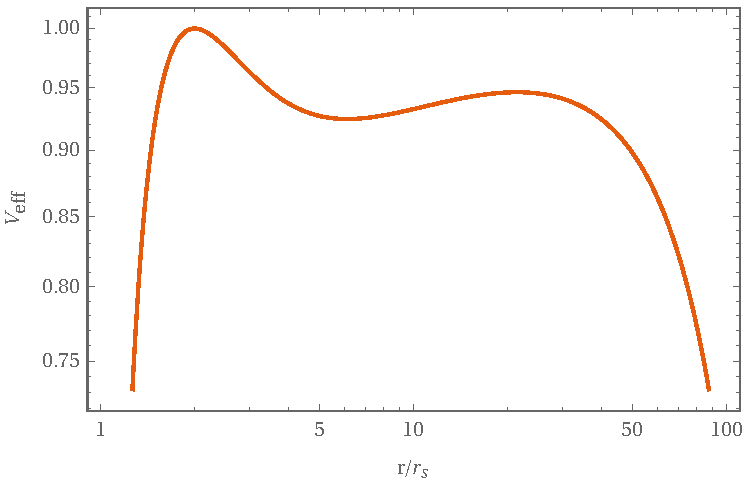
\includegraphics[scale=1]{Effective_Potential}
\end{center}
\caption{Effective potential for massive particle with parameters $\epsilon = 1$, $\mathcal{L} = 2$, $\Lambda = 10^{-4}$. }
\end{figure}

\renewcommand{\sh}[1]{\left( 1 - \frac{r_s}{#1} \right)}

\section*{2.}

For the Schwarzschild metric in coordinates $(t, r, \theta, \phi)$ which we label $(x^1, x^2, x^3, x^4)$,
\[ \d{s^2} = - \sh{r} c^2 \d{t^2} + \sh{r}^{-1} \d{r^2} + r^2 (\d{\theta^2} + \sin^2{\theta} \: \d{\phi^2} ) \]
We can use the formulas given for the Christoffel symbols and the definition,
\[ R^\rho_{\: \sigma \mu \nu} = \partial_\mu \Gamma^{\rho}_{\nu \sigma} - \partial_\nu \Gamma^\rho_{\mu \sigma} + \Gamma^\rho_{\mu \lambda} \Gamma^\lambda_{\nu \sigma} - \Gamma^\rho_{\nu \lambda} \Gamma^\lambda_{\mu \sigma} \]
to compute all independent components of the Riemann tensor. The nonzero Riemann tensor components are,
\begin{align*}
R_{1212} & = -R_{2112} = - R_{1221} = R_{2121} = - \frac{r_s}{r^3} 
\\
R_{1313} & = -R_{3113} = - R_{1331} = R_{3131} = \frac{(r - r_s)r_s}{2 r^2} 
\\
R_{1414} & = -R_{4114} = - R_{1441} = R_{4141} = \frac{(r - r_s)r_s \sin^2{\theta}}{2 r^2}
\\
R_{2323} & = -R_{3223} = - R_{2332} = R_{3232} = - \frac{r_s}{2(r - r_s)}
\\
R_{2424} & = -R_{4224} = - R_{2442} = R_{4242} = - \frac{r_s \sin^2{\theta}}{2(r - r_s)}
\\
R_{3434} & = -R_{4334} = - R_{3443} = R_{4343} = r r_s \sin^2{\theta}
\end{align*}
Then we may compute the invariant,
\[ R^{\alpha \beta \gamma \delta} R_{\alpha \beta \gamma \delta} = \frac{12 r_s^2}{r^6} \]

\section*{3.}
A Black Hole of mass $M$ has Schwarzschild radius,
\[ r_s = \frac{2MG}{c^2} \]
Consider a photon orbit with affine parameter $\lambda$ which must satisfy,
\[ u_\alpha u_\beta g^{\alpha \beta} = - \sh{r}^{-1} u_{t}^2 + \sh{r} u_r^2 + \frac{u_\phi^2}{r^2} = 0 \] 
Furthermore, because of the $t$ and $\phi$ Killing vectors the quantities $u_t = -E/c$ an $u_\phi = L$ are conserved along these geodesics. 
Now we use,
\[ \deriv{r}{\lambda} = u^r = g^{rr} u_r = \sh{r} u_r \]
to find that,
\[ \left( \deriv{r}{\lambda} \right)^2 = \frac{E^2}{c^2} - \sh{r} \frac{L^2}{r^2} \]
Now we rewrite,
\[ \left( \frac{c}{E} \deriv{r}{\lambda} \right)^2 = 1 - \sh{r} \frac{\alpha^2}{r^2} \]
and rescale $\lambda \mapsto E \lambda/c$ where,
\[ \alpha = \frac{Lc}{E} \]
is the angular parameter of the photon motion. Under this rescaling of the affine parameter the conserved quantities become,
\[ \sh{r} c \deriv{t}{\lambda} = 1 \quad \quad \quad \alpha = r^2 \deriv{\phi}{\lambda} \]
Thus we have the equation of motion,
\[ \deriv{r}{\lambda} = \sqrt{1 - \sh{r} \frac{\alpha^2}{r^2}} \]
which we may write as an energy equation,
\[ \frac{1}{2} \left( \deriv{r}{\lambda} \right)^2 + \frac{1}{2} \sh{r} \frac{\alpha^2}{r^2} = \frac{1}{2} \]
with effective potential,
\[ V(r) = \frac{1}{2} \sh{r} \frac{\alpha^2}{r^2} \]
Circular orbits may occur when $V'(r) = 0$. Consider,
\begin{align*}
V'(r) = \frac{1}{2} \deriv{}{r} \left[ \sh{r} \frac{\alpha^2}{r^2} \right] = \frac{1}{2} \frac{r_s \alpha^2}{r^4} - \sh{r} \frac{\alpha^2}{r^3} = \frac{3}{2} \frac{r_s \alpha^2}{r^4} - \frac{\alpha^2}{r^3}
\end{align*}
Therefore,
\[ V'(r) = 0 \iff \tfrac{3}{2} r_s \alpha^2 - \alpha^2 r = 0 \iff r = \tfrac{3}{2} r_s \]
Therefore, photon orbits occur at the photon sphere with radius, $r_p = \tfrac{3}{2} r_s$. For this orbit to occur we must also have $\dot{r} = 0$ and thus from the equation of motion,
\[ \sh{r_p} \frac{\alpha^2}{r_p^2} = 1 \]
which implies that,
\[ \alpha_p = \frac{3 \sqrt{3}}{2} r_s \]
Furthermore consider the stability given by the second derivative,
\[ V''(r) = \deriv{}{r} \left[ \frac{3}{2} \frac{r_s \alpha^2}{r^4} - \frac{\alpha^2}{r^3} \right] = - \frac{6 r_s \alpha^2}{r^5} + \frac{3 \alpha^2}{r^4} = - \frac{\alpha^2}{r^4} \left(\frac{3 r_s}{r} - 1 \right) \]
At the photon sphere $r < 3 r_s$ and thus $V''(r) < 0$ so the orbits are unstable. This unstable orbit occurs at a radius of,
\[ r_p = \tfrac{3}{2} r_s = \frac{3 MG}{c^2} \]
Furthermore,
\[ \dot{\phi} = \frac{u^\phi}{u^t} = \frac{c \alpha}{r_p^2} \left( 1 - \frac{r_s}{r} \right) = \frac{2}{3 \sqrt{3}} \frac{c}{r_s}  \]
and therefore, the period of the orbit is,
\[ P = 3 \sqrt{3} \pi \left( \frac{r_s}{c} \right) \]

\section*{4.}

Consider a massive particle with mass $m$ in Schwarzschild space-time with geodesic four-velocity satisfying,
\[ g^{\alpha \beta} u_\alpha u_\beta = - \sh{r}^{-1} u_t^2 + \sh{r} u_r^2 + \frac{u_\phi^2}{r^2} = - c^2 \]
Because of the killing vectors we have conserved quantities, 
\[ u_t = - \frac{E}{mc} \quad \quad u_\phi = \frac{L}{m} \]
Now using the fact that,
\[ \dot{r} = \deriv{r}{\tau} = u^r = g^{rr} u_r = \sh{r} u_r \]
we find the radial equation,
\[ \frac{\dot{r}^2}{c^2} + \sh{r} \left(1 + \frac{L^2}{m^2 c^2 r^2} \right) = \left( \frac{E}{mc^2} \right)^2  \]
Therefore, define dimensionless parameters,
\[ \ell = \frac{L}{mcr_s} \quad \quad \epsilon = \frac{E}{mc^2} \]
And rescale $\tau \mapsto c \tau$ which gives an energy equation,
\[ \frac{1}{2} \dot{r}^2 + \frac{1}{2} \sh{r} \left(1 + \ell^2 \left( \frac{r_s}{r} \right)^2 \right) = \frac{1}{2} \epsilon^2  \]
with effective potential,
\[ V(r) = \frac{1}{2} \sh{r} \left(1 + \ell^2 \left( \frac{r_s}{r} \right)^2 \right) \]
In the case that the particle starts at $r = \infty$ with $v_\infty \ll c$ then,
\[ \epsilon = 1 + \frac{1}{2} \left( \frac{v_\infty}{c} \right)^2 + O(v_\infty / c) \]
The turning points of this orbit occur when $V(r) = \tfrac{1}{2} \epsilon^2$. Therefore, to first-order in $v_\infty / c$ we need to solve the equation,
\[ \sh{r} \left(1 + \ell^2 \left( \frac{r_s}{r} \right)^2 \right) = 1 + \left( \frac{v_\infty}{c} \right)^2 \]
The particle can fall into the black hole if the particle has enough energy to pass the barrier of the inner unstable orbit i.e. the inner radius when $V'(r) = 0$. Written in terms of the variable $u = r_s / r$ we consider $V'(u) = 0$ which happens when,
\[ \deriv{}{u} \left[ (1 - u) (1 + \ell^2 u^2) \right] = -(1 + \ell^2 u^2) + 2 \ell^2 (1 - u)u = 0 \]
And thus,
\[ 3 u^2 \ell^2 - 2 \ell^2 u + 1 = 0 \] 
so the extrema occur at,
\[ u = \tfrac{1}{3} (1 \pm \sqrt{1 - 3 \ell^{-2}}) \quad \text{thus} \quad  r = r_s \ell^2 \left( 1 \pm \sqrt{1 - 3 \ell^{-2}} \right) \]
Now note that when $\ell = 2$ we have $r_{\text{in}} = 2 r_s$ in which case,
\[ 2 V(r_{\text{in}}) = (1 - \tfrac{1}{2})(1 + 1) = 1 \]
Therefore, to zeroth-order in $v_\infty / c$ we have $\ell_{\text{min}} = 2$ because for this value the pericenter of the orbit lies exactly at the innermost maximum of the potential, the radius of unstable circular orbits, so any lower $\ell$ will result in the particle energy being above the centrifugal barrier. For $\ell = \ell_{\text{max}}$ the particle comes to rest at $r = 2r_s$, the radius of inner unstable circular orbits for that fixed angular momentum, since it is a maximum of the potential and there the particle will spiral onto this radius making an infinite number of turns around the black hole. However, in reality, this will not occur because such an orbit is unstable and will eventually fall into the black hole or be flung off to infinity. 
\bigskip\\
Now the pericenter is the outermost solution to,
\[ V(r) = \tfrac{1}{2} \epsilon^2 \iff \sh{r} \left(1 + \ell^2 \left( \frac{r_s}{r} \right)^2 \right) = 1 \]
In terms of the variable $u = r_s / r$ this is equivalent to the cubic equation,
\[ (1 - u)(1 + \ell^2 u^2) - 1 = 0 \iff  \ell^2 u^3 - \ell^2 u^2 + u = 0 \]
Thankfully there is no constant term and the solution $u = 0$ is the initial condition at $r = \infty$ meaning that the remaining solutions are to the quadratic,
\[ \ell^2 u^2 - \ell^2 u + 1 = 0 \]
which has solutions,
\[ u = \tfrac{1}{2} (1 \pm \sqrt{1 - 4 \ell^{-2}}) \quad \text{thus} \quad r = \tfrac{1}{2} \ell^2 (1 \pm \sqrt{1 - 4 \ell^{-2}}) \]
Then the pericenter is the largest such radial solution,
\[ r_p = \tfrac{1}{2} r_s \ell^2 (1 + \sqrt{1 - 4 \ell^{-2}}) \]
Thus we see clearly that $\ell \ge \ell_{\text{min}} = 2$ for such a turning-point to exist. 

\section*{5.}

Consider a star moving on a parabolic orbit with orbital energy $\epsilon = 1$ about a supermassive Schwarzschild black hole with dimensionless angular momentum $\ell = 3$. We have shown that the pericenter is at,
\[ r_p = \tfrac{9}{2} r_s (1 + \sqrt{1 - 4/9}) = \tfrac{3}{2} r_s (3 + \sqrt{5}) \]  

\begin{enumerate}
\item At the pericenter, we have $u^r = u^\theta = 0$ and,
\[ u^t = g^{tt} u_t = - g^{tt} E/c = \sh{r_p}^{-1} c  \quad \quad u^\phi = g^{\phi \phi} u_{\phi} = r_p^{-2} \ell r_s c \]
Then we have,
\[ u^\alpha = (\tfrac{3}{2}(3 - \sqrt{5}) c, 0, 0, \tfrac{1}{6}(7 - 3 \sqrt{5}) c/r_s) \]

\begin{remark}
I use the notation $\bf{e}_\mu$ for the Schwarzschild basis vectors and $\bf{o}_\mu$ for the basis vectors in another frame. These can be written in components the Schwarzschild basis via $(o_\beta)^\alpha = \bf{o}_\beta \cdot \bf{e}^\alpha$ (which is the quantity notated as $e_{(\beta)}^\alpha$ in the problem statement). 
\end{remark}

\item We first need to set up the local inertial rest frame of the star at its pericenter. First we have $c \bf{o}_t = \bf{u}$, the four velocity of the star, because in its locally inertial rest frame, the star's four-velocity is parallel to the time direction. Furthermore, we set,
\[ \bf{o}_r = \sqrt{1 - \frac{r_s}{r_p}} \bf{e}_r \]
such that $\bf{o}_t \cdot \bf{o}_r = u^r \bf{e}_r \cdot \bf{o}_r = 0$ since $u^r = 0$ and $(\bf{o}_t)^2 = -1$ and $(\bf{o}_r)^2 = 1$.
\bigskip\\
Now consider a radial point on the star i.e. one with displacement vector $\bf{S} = S \bf{o}_r$ i.e. in local components $S^r = S$ and $S^i = 0$ otherwise. The tidal acceleration is given by,
\[ \nderiv{2}{S^i}{t} = - R_{\alpha \beta \gamma \delta} (o_i)^\alpha u^\beta (o_k)^\gamma u^\delta S^k \]
In the radial direction, plugging in $\bf{S} = S \bf{o}_r$,
\[ \nderiv{2}{S^r}{t} = - R_{\alpha \beta \gamma \delta} (o_r)^\alpha u^\beta (o_r)^\gamma u^\delta S \]
However, $(o_r)^\alpha = (0,1,0,0) \sqrt{1 - \frac{r_s}{r_p}}$ and $u^r = u^\theta = 0$ so using the nonzero components of the Riemann tensor, this simplifies to,
\[ \nderiv{2}{S^r}{t} = - S \sh{r_p} R_{rtrt} (u^t)^2 - S \sh{r_p} R_{r\phi r \phi} (u^\phi)^2 \]
Plugging in the components of the Riemann tensor and four-velocity,
\begin{align*}
\nderiv{2}{S^r}{t} & = S \sh{r_p} \frac{r_s}{r_p^3} \sh{r_p}^{-2} c^2 + S \sh{r_p} 
\frac{r_s}{2(r_p - r_s)} \cdot \frac{r_s^2 \ell^2}{r_p^4} c^2
\\
& = S \frac{r_s}{r_p^3} \sh{r_p}^{-1} c^2 + S\frac{r_s^3 \ell^2}{2r_p^5} c^2
\end{align*}

Now plugging in $\ell = 3$ and $r_p/r_s = \frac{3}{2} (3 + \sqrt{5})$ we have,
\[ \nderiv{2}{S^r}{t} = 0.0025157 \frac{Sc^2}{r_s^2} = 0.0025157 \frac{S c^6}{4 M^2 G^2} \]
Plugging in $S = 10^{11} \: \mathrm{cm}$ and $M = 2 \times 10^{40} \: \mathrm{g}$ we obtain,
\[ \nderiv{2}{S^r}{t} = 256 \: \mathrm{m} / \mathrm{s}^2 \]
To determine whether the star is tidally disrupted, we need to compute the gravitational acceleration of the star itself at the surface and determine if this exceeds the tidal acceleration. Because the star is large compared to its mass we may do this classically,
\[ \nderiv{2}{S^r}{t} = - \frac{M_sG}{S^2} \] 
For the value $M_s = 2 \times 10^{33} \: \mathrm{g}$ we have,
\[ \nderiv{2}{S^r}{t} = - 133 \: \mathrm{m} / \mathrm{s}^2 \]
Since the outward tidal acceleration exceeds the inwards gravitational attraction, the star is disrupted by tidal forces at the pericenter. 
\end{enumerate}

\section*{6.}

Consider the equation of motion for a photon,
\[ \frac{1}{2} \left( \deriv{r}{\lambda} \right)^2 + \frac{1}{2} \sh{r} \frac{\alpha^2}{r^2} = \frac{1}{2} \]
We need to find the minimal angular parameter $\alpha$ such that inwards traveling photons do not cross the even horizon. This cutoff occurs for photons which graze the photon sphere. To see this recall that the photon effective potential has a unique extremum at $r = r_p = \tfrac{3}{2} r_s$ which corresponds to a maximum of the potential at the photon sphere. Therefore an inwards photon orbit will cross the even horizon exactly if the potential is low enough for it to cross the photon sphere barrier and otherwise the orbit will have a turning point at some $r > r_p$. Therefore, the condition for the photon to escape is,
\[ V(r_p) > \frac{1}{2} \iff \sh{r_p} \frac{\alpha^2}{r_p^2} > 1 \iff \alpha > \frac{3 \sqrt{3}}{2} r_s \]
we write this condition as,
\[ \alpha > \alpha_{\text{crit}} \quad \text{where} \quad \alpha_{\text{crit}} = \frac{3 \sqrt{3}}{2} r_s \]
For an outwards emitted photon to escape (if emitted within the photon sphere) the potential barrier must be low enough for the photon to cross otherwise there will be a turning point within the photon sphere and the photon will reverse course and cross the event horizon. Thus in the outwards moving case for $r \le r_p$ the condition for escape is,
\[ \alpha < \alpha_{\text{crit}} \]
Now we need to compute the angles at which these critical photons are emitted \textit{in the proper frame of the emitter}. Using our above formulas, in terms of Schwarzschild coordinate basis vectors, the photon four momentum is,
\[ \bf{p} = \frac{E_\infty}{c} \left( \sh{r}^{-1} \bf{e}_t \pm \sqrt{1 - \sh{r} \frac{\alpha^2}{r^2}} \bf{e}_r + \frac{\alpha}{r^2} \bf{e}_\phi \right) \]
Now we need to consider the basis vectors of the proper frame of the emitter at the location of the emitter. We set,
\begin{align*}
\bf{o}_t & = \bf{e}_t \sh{r}^{-\frac{1}{2}}
\\
\bf{o}_r & = \bf{e}_r \sh{r}^{\frac{1}{2}}
\\
\bf{o}_x & = \bf{e}_\phi (r \sin{\theta})^{-1}
\\
\bf{o}_y & = \bf{e}_{\theta} r^{-1}
\end{align*}
Such that, in the new frame,
\[ g'_{\mu \nu} = \bf{o}_\mu \cdot \bf{o}_\nu = \eta_{\mu \nu} \]
Since the new frame is locally Minkowski, the proper velocities are simply the coordinate velocities,
\begin{align*}
\frac{v_x}{c} & = \deriv{x}{ct} = \frac{\deriv{x}{\lambda}}{\deriv{ct}{\lambda}} = \frac{p^x}{p^t} = - \frac{p_x}{p_t} = - \frac{\bf{p} \cdot \bf{o}_x}{\bf{p} \cdot \bf{o}_t} 
\\
& = \frac{\alpha}{r} \sqrt{1 - \frac{r_s}{r}} 
\end{align*}
Therefore, for a given photon momentum $\bf{p}$ the apparent angle of emission (with respect to the center of the black hole) in the emitter frame is,
\[ \sin{\psi} = \frac{\alpha}{r} \sqrt{1 - \frac{r_s}{r}} \]
Therefore, the critical angle under which all photons are captured across the event horizon is,
\[ \sin{\psi_{\text{c}}} = \frac{\alpha_{\text{c}}}{r} \sqrt{1 - \frac{r_s}{r}} \]
We choose the branch $0 \le \psi \le \frac{\pi}{2}$ for $r > r_p$ because in that range the critical photon is emitted inwards towards the black hole and the branch $\frac{\pi}{2} \le \psi \le \pi$ for $r \le r_p$ because in this range the critical photons are emitted away from the black hole (all photons emitted towards the black hole are absorbed). Now the solid angle into which the light is absorbed is,
\[ \Omega = 2\pi (1 - \cos{\psi_{\text{c}}}) \]
Therefore, for an isotropic source, the fraction of light absorbed by the black hole is,
\[ \frac{\Omega}{4 \pi} = \tfrac{1}{2} (1 - \cos{\psi_{\text{c}}}) \]
Now to compute the cosine note that,
\[ \cos{\psi} = -\frac{v_r}{c} = \frac{\bf{p} \cdot \bf{o}_r}{\bf{p} \cdot \bf{o}_t} = \mathrm{sign}{(r - r_p)} \sqrt{1 - \sh{r} \frac{\alpha^2}{r^2}}  \] 
We take the negative sign for $r < r_p$ when we choose positive radial velocity corresponding to outgoing critical photons and the positive sign for $r > r_p$ when we choose negative radial velocity corresponding to incoming critical photons.
It is an encouraging check that,
\[ \sin^2{\psi} + \cos^2{\psi} = \sh{r} \frac{\alpha^2}{r^2} + 1 - \sh{r} \frac{\alpha^2}{r^2} = 1 \]
and therefore $v_x^2 + v_r^2 = c^2$ so photons do indeed travel at the speed of light as they must in this locally inertial frame. Therefore, the fraction of the light which is absorbed by falling across the event horizon is,
\[ \frac{\Omega}{4 \pi} = \frac{1}{2} \left(1 - \mathrm{sign}{(r - r_p)} \sqrt{1 - \sh{r} \frac{\alpha_{\text{c}}^2}{r^2}} \right) \]
Now we consider the limit $r \gg r_s$ then,
\[ \sin{\psi_{\text{c}}} \approx \frac{\alpha_{\text{c}}}{r} \]
and thus, at large radii, the black hole has an apparent radius of,
\[ r_{\text{app}} = \alpha_{\text{c}} = \frac{3 \sqrt{3}}{2} r_s \approx 2.60 r_s \]
Likewise, in the large $r \gg r_s$ regime we have,
\[ \frac{\Omega}{4 \pi} \approx \frac{\alpha_{\text{c}}^2}{4 r^2} = \frac{1}{4} \left( \frac{r_{\text{app}}}{r} \right)^2 = \frac{27}{16} \left( \frac{r_s}{r} \right)^2 \]
which is approximately the fraction of the sky covered by a disc of radius $r_{\text{app}}$ viewed at a large distance $r \gg r_{\text{app}}$ since it is the area of the disc $A = \pi r_{\text{app}}^2$ divided by the total area of the sky sphere $4 \pi r^2$. 
\begin{figure}
\begin{center}
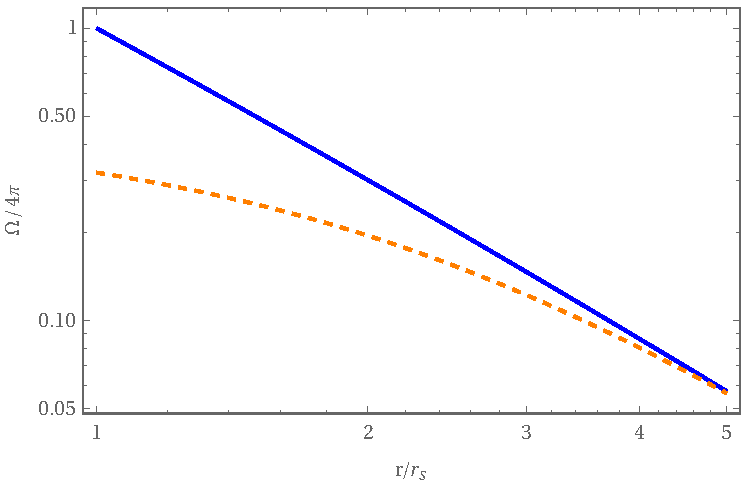
\includegraphics[scale=1]{Apparent_Size}
\end{center}
\caption{Apparent size measured as fraction of total area of sky subtended of a Schwarzschild black hole as a function of dimensionless radius $r / r_s$. Dashed line shows the classical apparent size of an object with radius $r_{\text{app}}$. }
\end{figure}


\section*{7.}

Consider a fixed observer near a Schwarzschild black hole of mass $M$ (and thus Schwarzschild radius $r_s$) at constant coordinates $(r_*, \theta_*, \phi_*)$ which drops a beacon radially into the black hole. 

\begin{enumerate}
\item Using the metric restricted to radial motion $(\d{\theta} = \d{\phi} = 0$) we find,
\[ \left( \deriv{\tau}{t} \right)^2 = \sh{r} c^2 - \sh{r}^{-1} \left( \deriv{r}{t} \right)^2 \]
However, recall that,
\[ E = \sh{r} mc^2 \deriv{t}{\tau} \]
is a conserved quantity due to the time-like Killing vector. Therefore,
\[ \frac{\dot{r}}{c} = \sh{r} \sqrt{1 - \sh{r} \left( \frac{mc^2}{E} \right)^2 } \]
Now we know that initially the beacon is at rest when $r = r_*$ meaning that,
\[ E =  mc^2 \sqrt{1 - \frac{r_s}{r_*}} \]
which implies that,
\[ \frac{\dot{r}}{c} = \sh{r} \sqrt{1 - \frac{\sh{r}}{\sh{r_*}}} \]
which may be simplified to,
\[ \frac{\dot{r}}{c} = \sh{r} \sqrt{\frac{r_s}{r}\cdot \frac{r_* - r}{r_* - r_s}} \]

\item For a local fixed observer at position $(r, \theta, \phi)$ we have observer coordinates,
\[ \d{t_{\text{obs}}^2} = \sh{r} \d{t^2} \quad \quad \quad \d{r_{\text{obs}}^2} = \sh{r}^{-1} \d{r^2} \]
Therefore, 
\[ v_{\text{obs}} = \frac{\d{r_{\text{obs}}}}{\d{t_{\text{obs}}}} = \sh{r}^{-1} \dot{r} = c \sqrt{\frac{r_s}{r}\cdot \frac{r_* - r}{r_* - r_s}} \]
Now in the limit $r \to r_s$ we find that $v_{\text{obs}} \to c$.

\item The energy of the photon is the time component of its four-momentum in a local observer frame. We have previously written down the photon four momentum and local observer frame. Thus,
\[ E = c \eta^{00} \bf{p} \cdot \bf{o}_t = - \bf{p} \cdot \bf{o}_t = E_\infty \sh{r}^{-\frac{1}{2}} \]
In a locally Minkowski frame then the wavelength of the light is related via,
\[ \lambda = \frac{hc}{E} = \lambda_{\infty} \sqrt{1 - \frac{r_s}{r}} \]
Therefore for a given light beam emitted at $r_{\text{em}}$ with wavelength $\lambda_{\text{em}}$ \textit{in the local observer frame} and observed at $r_*$ with wavelength $\lambda_{\text{obs}}$ we have,
\begin{align*}
\lambda_{\text{em}} &= \lambda_{\infty} \sqrt{1 - \frac{r_s}{r_{\text{em}}}}
\\
\lambda_{\text{obs}} &= \lambda_{\infty} \sqrt{1 - \frac{r_s}{r_*}}
\end{align*}
Therefore,
\[ 1 + z = \frac{\lambda_{\text{obs}}}{\lambda_{\text{em}}} = \sqrt{\frac{r_{\text{em}}}{r_*} \cdot \frac{r_* - r_s}{r_{\text{em}} - r_s}} \]
However, in the current case, the emitter is not in the local observer frame because it is moving with respect to the black hole. Therefore we need to set up a local rest frame to compute the energy of the photon. Note that the local time-like basis vector will be $c \bf{o}_t = \bf{u}$ the four-velocity of the emitter frame. This is because the four-velocity of the emitter should be exactly $c \bf{o}_t$ in this local rest frame corresponding to the fact that it is at rest in this frame. Therefore,
\[ E = c \eta^{tt} \bf{p} \cdot \bf{o}_t = - \bf{p} \cdot \bf{u} = - p_\alpha u^\alpha \]
This is clearly an invariant so calculating it in the rest frame in which $u^\alpha = (c,0,0,0)$ simply gives $E = p^t c$ as expected. Therefore, using the formula for photon momentum, 
\[ \bf{p} = \frac{E_\infty}{c} \left( \sh{r}^{-1} \bf{e}_t + \bf{e}_r \right) \]
and the four-velocity of the emitter,
\[ \bf{u} = \deriv{ct}{\tau} \bf{e}_t + \deriv{r}{\tau} \bf{e}_r = c\sqrt{1 - \frac{r_s}{r_*}} \left( \sh{r}^{-1}  \bf{e}_t - \sqrt{\frac{r_s}{r} \cdot \frac{r_* - r}{r_* - r_s}} \: \bf{e}_r \right) \]
then gives,
\[ E = E_{\infty} \sh{r}^{-1} \sqrt{1 - \frac{r_s}{r_*}} \left( 1  + \sqrt{\frac{r_s}{r} \cdot \frac{r_* - r}{r_* - r_s}} \right) \]
Then as before,
\[ \lambda = \lambda_{\infty} \sh{r} \sh{r_*}^{-\frac{1}{2}} \left( 1  + \sqrt{\frac{r_s}{r} \cdot \frac{r_* - r}{r_* - r_s}} \right)^{-1} \]
This is the actual wavelength observed in the emitter frame meaning that,
\[ 1 + z = \frac{\lambda_{\text{obs}}}{\lambda_{\text{em}}} = \left( \frac{r}{r_*} \cdot \frac{r_* - r_s}{r - r_s} \right) \cdot  \left( 1  + \sqrt{\frac{r_s}{r} \cdot \frac{r_* - r}{r_* - r_s}} \right)  \]


\item For light ray emitted radially, we find from the null geodesic condition,
\[ \sh{r} c^2 \d{t^2} - \sh{r}^{-1} \d{r^2} = 0 \]
and therefore,
\[ \dot{r} = c \sh{r} \]
Integrating this we equation we find,
\[ c \Delta t = (r_* - r_{\text{em}}) + r_s \log{\left( \frac{r_* - r_s}{r_{\text{em}} - r_s}\right)} \]
This is the global time it takes for the light beam to traverse from $r_{\text{em}}$ to $r_*$. Then the observer time at radius $r_*$ is,
\[ c \Delta t_{\text{obs}} = \sqrt{1 - \frac{r_s}{r_*}} \left[(r_* - r_{\text{em}}) + r_s \log{\left( \frac{r_* - r_s}{r_{\text{em}} - r_s}\right)} \right] \]
This is the light travel time however we also need to know the time it takes for the emitter to fall from the initial point $r_*$ to the radius $r_{\text{em}}$. We need to solve,
\[ \frac{\dot{r}}{c} = -\sh{r} \sqrt{\frac{r_s}{r} \cdot \frac{r_* - r}{r_* - r_s}} \]
This is too difficult to solve exactly but we only need to know the asymptotic behavior. Consider $r = r_s(1 + \epsilon)$ then we can expand,
\[ \dot{\epsilon} = - \frac{c}{r_s} \left( \epsilon + \frac{1}{2} \sh{r_*}^{-1} \epsilon^2 + O(\epsilon) \right) \]
To first-order we have,
\[ \epsilon = \epsilon_0 e^{- \frac{c}{r_s} t} \]
which implies that, in global time,
\[ ct = r_s \log{\left( \frac{r_* - r_s}{r_{\text{em}} - r_s} \right)} \]
This has the same asymptotic form as the light travel time because as the emitter approaches the horizon it approaches the speed of light in  local coordinates. Therefore, asymptotically, the observer time at which a light beam originating at radius $r_{\text{em}}$ is received is,
\[ c t_{\text{obs}} = 2 r_s \sqrt{1 - \frac{r_s}{r_*}} \log{\left( \frac{r_* - r_s}{r_{\text{em}} - r_s} \right)} \]

\item In the late time regime we write $r = r_s(1 + \epsilon)$ for small $\epsilon$. When we expand to first-order in small $\epsilon$ we  find that,
\[ c t_{\text{obs}} = -2 r_s \sqrt{1 - \frac{r_s}{r_*}} \log{\epsilon} + C \]
Furthermore,
\[ 1 + z = \sh{r_*} (1 + \epsilon^{-1}) \cdot \left(1 + \sqrt{(1 - \epsilon) \cdot \left(1 - \frac{r_s}{r_* - r_s} \epsilon \right)} \right) = \frac{2}{\epsilon} \sh{r_*} + O(1)   \]
Therefore, in the limit $\epsilon \to 0$ i.e. $r \to r_s$ which corresponds to large times we have,
\[ z \approx \frac{2}{\epsilon} \sh{r_*} \quad \quad c t_{\text{obs}} \approx - \sh{r_*} r_s \log{\epsilon} \]
Therefore,
\[ z \approx 2 \sh{r_*} e^{t_{\text{obs}} / T} \quad \text{where} \quad T = \frac{2r_s}{c} \sqrt{1 - \frac{r_s}{r}} = \frac{4 MG}{c^3} \sqrt{1 - \frac{2 MG}{r_* c^2}} \]
\end{enumerate}

\section*{8.}

Consider the Schwarzschild metric,
\[ \d{s^2} = - \sh{r} c^2 \d{t^2} + \sh{r}^{-1} \d{r^2} + r^2 ( \d{\theta^2} + \sin^2{\theta} \: \d{\phi^2} )  \]
specifically in the interior of the event horizon $r < r_s$. Massive particles must traverse paths with positive proper time i.e. $\d{s^2} < 0$. This implies that,
\[  \left( \frac{r_s}{r} - 1 \right)^{-1} \d{r^2}  >  \left( \frac{r_s}{r} - 1 \right) c^2 \d{t^2} +  r^2 ( \d{\theta^2} + \sin^2{\theta} \: \d{\phi^2} ) \]
In the region $r < r_s$ all these quantities are positive. Furthermore,
\[ \d{\tau^2} = -\left( \frac{r_s}{r} - 1 \right) \d{t^2} + \left( \frac{r_s}{r} - 1 \right)^{-1} c^{-2} \d{r^2} - r^2 c^{-2} ( \d{\theta^2} + \sin^2{\theta} \: \d{\phi^2} ) \]
Therefore,
\[ \left( \frac{r_s}{r} - 1 \right)^{-1} \left( \deriv{r}{\tau} \right)^2 = c^2 + \left( \frac{r_s}{r} - 1 \right) c^2 \d{t^2} + r^2 ( \d{\theta^2} + \sin^2{\theta} \: \d{\phi^2} ) \]
Since all these quantities are positive, this implies that,
\[ \left( \frac{r_s}{r} - 1 \right)^{-1} \left( \deriv{r}{\tau} \right)^2 \ge c^2 \]
which is equivalent to,
\[ \left| \deriv{r}{\tau} \right| \ge c \sqrt{\frac{r_s}{r} - 1} \]
\bigskip\\
This inequality implies that the maximum lifetime of a particle before it reaches the singularity at $r = 0$ must correspond to motion which saturates this inequality (otherwise the radius decreases more quickly with proper time). Consider a trajectory which saturates this inequality,
\[ \deriv{r}{\tau} = - c \sqrt{\frac{r_s}{r} - 1} \]
Then,
\[ \tau = \frac{1}{c} \int_{0}^{r_s} \frac{\d{r}}{\sqrt{\frac{r_s}{r} - 1}} =  \frac{1}{c} \int_0^{r_s} \frac{r^{\frac{1}{2}} \d{r}}{\sqrt{r_s - r}} \]
Consider the substitution $r = r_s \sin^2{t}$. Then $\d{r} = 2 r_s \cos{t} \sin{t} \: \d{t}$ so we find,
\[ \tau_{\text{max}} = \frac{2r_s}{c} \int_0^{\frac{\pi}{2}} \frac{\sin^2{t} \cos{t}}{\sqrt{1 - \sin^2{t}}} \d{t} = \frac{2 r_s}{c} \int_0^{\frac{\pi}{2}} 2 \sin^2{t} \d{t} = \frac{r_s \pi}{2c} \]
This is the maximal lifetime, any other trajectory inside the event horizon will end on the singularity and have proper time less than $\tau_{\text{max}}$. We may write this maximal time as,
\[ \tau_{\text{max}} = \frac{\pi MG}{c^3} = 15.5 \cdot \left( \frac{M}{M_{\odot}} \right) \:\text{ms} \]
Finally, we must show that free fall geodesics with $E \to 0$ do indeed saturate this inequality and thus are the maximal lifetime trajectories. Consider the radial equation specialized with $L = 0$,
\[ \left( \deriv{r}{\tau} \right)^2 + c^2 \sh{r} = \frac{E^2}{m^2 c^2} \]
Therefore,
\[ \left| \deriv{r}{\tau} \right| = c \sqrt{\left( \frac{E}{mc^2} \right)^2 + \left( \frac{r_s}{r} - 1 \right)} \]
Therefore, in the limit $E \to 0$ we have,
\[ \left| \deriv{r}{\tau} \right| = c \sqrt{\frac{r_s}{r} - 1} \]
saturating the inequality and thus showing that this trajectory maximizes proper time along the path until hitting the singularity.

\end{document}